%===============================================================================
\chapter{Turbulence and Fluid Dynamics}
\label{ch:fluids}
%===============================================================================

Fluid turbulence represents one of the most spectacular manifestations of scale hierarchy in physics. Energy injected at large scales cascades through an inertial range before being dissipated at small scales. The RG provides the natural language for describing this multi-scale structure, and this chapter applies the \textbf{algebraic}, \textbf{geometric}, and \textbf{analytic} framework of Parts I and II to turbulence.

\marginnote{Turbulence involves fluctuations over a vast range of scales, making it a perfect arena for RG methods.}

This chapter is organized around three themes:

\textbf{Algebraic structure.} The RG for turbulence is the action of the dilation group on a theory space parametrized by effective viscosity, forcing spectrum, and higher couplings. Beta functions are the Lie algebra generators; fixed points are where these generators vanish. The \textbf{Kolmogorov fixed point} describes universal scaling in the inertial range.

\textbf{Taxonomy of approaches.} Multiple RG approaches exist---Yakhot-Orszag direct coarse-graining, McComb iterative averaging, MSR-JD field theory, and functional RG. We show these are different implementations of the same geometric structure. Remarkably, \textbf{closure methods} like Kraichnan's Direct Interaction Approximation can be reinterpreted as \emph{fixed points} (analogous to the Gaussian fixed point in $\phi^4$ theory) from which the true turbulent state is reached by RG flow.

\textbf{Analytical structure.} Applying Part II's framework, we examine the divergent nature of turbulence perturbation theory. The series is generically Gevrey-1; Borel singularities correspond to coherent structures and intermittent events; and \textbf{resurgence} may explain the anomalous dimensions responsible for intermittency corrections.

Throughout, we make essential contact with Barenblatt's theory of intermediate asymptotics, the conformal structure of fluid equations, and the deep parallels with critical phenomena.

%-------------------------------------------------------------------------------
\section{The Navier-Stokes Equations}
\label{sec:navier_stokes}
%-------------------------------------------------------------------------------

The incompressible Navier-Stokes equations describe the motion of a viscous fluid:
\begin{align}
\frac{\partial \mathbf{u}}{\partial t} + (\mathbf{u} \cdot \nabla)\mathbf{u} &= -\frac{1}{\rho}\nabla p + \nu \nabla^2 \mathbf{u} + \mathbf{f}, \label{eq:navier_stokes}\\
\nabla \cdot \mathbf{u} &= 0. \label{eq:incompressible}
\end{align}

Here $\mathbf{u}(\mathbf{x}, t)$ is the velocity field, $p$ the pressure, $\rho$ the density, $\nu$ the kinematic viscosity, and $\mathbf{f}$ an external forcing.

\subsection{Scale Identification}

Following Step 1 of the recipe, we identify the key scales. The integral scale $L$ characterizes the largest eddies where energy is injected, typically set by the geometry of the flow or the forcing mechanism. The Kolmogorov scale $\eta = (\nu^3/\varepsilon)^{1/4}$ characterizes the smallest eddies where viscous dissipation dominates, with $\varepsilon$ the energy dissipation rate per unit mass.

The corresponding velocity scales are the large-scale velocity $U$ at the integral scale and the Kolmogorov velocity $u_\eta = (\nu \varepsilon)^{1/4}$ at the dissipation scale. The Reynolds number $Re = UL/\nu$ measures the scale separation: for $Re \gg 1$, there is a wide inertial range $\eta \ll r \ll L$ where neither injection nor dissipation dominates. It is in this inertial range that universal scaling behavior emerges.

\marginnote{The Reynolds number is the control parameter analogous to $\rho$ in the Lorenz system or inverse temperature in statistical mechanics.}

%-------------------------------------------------------------------------------
\section{The Geometric Framework for Turbulence}
\label{sec:turb_geometry}
%-------------------------------------------------------------------------------

Before examining specific RG approaches to turbulence, we establish the geometric framework developed in Part I. This provides a unified language for comparing different methods and reveals deep structural similarities across approaches.

\subsection{Theory Space for Turbulence}

\marginnote{Theory space for turbulence is infinite-dimensional in principle, but tractable truncations exist.}

The \textbf{theory space} $\MM$ for turbulence consists of all possible effective descriptions of the velocity field statistics at a given scale. What are the coordinates on this space?

\textbf{Minimal parametrization.} For homogeneous, isotropic turbulence with power-law forcing, the essential parameters are:
\begin{itemize}
\item $\nu_{\text{eff}}$: the effective (eddy) viscosity
\item $D_0$: the forcing amplitude
\item $y$: the forcing spectrum exponent (for $\langle f f \rangle \sim k^y$)
\end{itemize}

This gives a finite-dimensional theory space $\MM \simeq \RR^+ \times \RR^+ \times \RR$ with coordinates $g = (\nu_{\text{eff}}, D_0, y)$.

\textbf{Extended parametrization.} A more complete description includes:
\begin{itemize}
\item Higher couplings $\lambda_n$ for nonlinear terms $(\mathbf{u} \cdot \nabla)^n \mathbf{u}$
\item Forcing correlation structure beyond power-law
\item Anisotropy parameters
\end{itemize}

In the field-theoretic approach (Section~\ref{sec:msr_jd}), theory space becomes the space of all operators consistent with the symmetries---analogous to the operator space in QFT.

\subsection{The Beta Function as Lie Algebra Generator}

The RG transformation acts on theory space by coarse-graining: integrating out velocity fluctuations at scales smaller than some cutoff $\ell$ while preserving the form of the effective equations. This defines a \textbf{flow} on $\MM$.

\marginnote{The beta function is the infinitesimal generator of the coarse-graining flow---the Lie algebra element that generates the RG group action.}

The \textbf{beta functions} are the components of the vector field generating this flow:
\begin{equation}
\frac{\dd g^i}{\dd s} = \beta^i(g), \quad s = \ln(\ell/\ell_0)
\end{equation}
where $s$ is the logarithmic scale parameter (analogous to $\ln \mu$ in QFT).

For the Yakhot-Orszag parametrization, the beta functions take the form (derived in Section~\ref{sec:ns_rg}):
\begin{align}
\beta_\nu &= (z - 2)\nu + \frac{A D_0}{\nu^2} + O(D_0^2/\nu^5) \label{eq:beta_nu}\\
\beta_{D_0} &= (y + 4 - 2z) D_0 \label{eq:beta_D}
\end{align}
where $z$ is the dynamical exponent and $A$ is a geometric constant.

\textbf{Lie algebra interpretation.} In the language of Chapter~\ref{ch:rg_geometry}, the beta function $\boldsymbol{\beta} = \beta^i \partial/\partial g^i$ is an element of the Lie algebra $\mathfrak{g}$ of the RG group. The RG transformation is the exponential map:
\begin{equation}
g(s) = \exp(s \cdot \boldsymbol{\beta}) \cdot g(0)
\end{equation}
This is exact; the beta function \emph{generates} the finite transformation.

\subsection{Fixed Points and Kolmogorov Scaling}

A \textbf{fixed point} $g^* \in \MM$ satisfies $\boldsymbol{\beta}|_{g^*} = 0$. At a fixed point, the theory is exactly scale-invariant.

\marginnote{The Kolmogorov fixed point is the turbulent analog of the Wilson-Fisher fixed point in critical phenomena.}

From equations~\eqref{eq:beta_nu}--\eqref{eq:beta_D}, the fixed point conditions are:
\begin{align}
\beta_{D_0} = 0 &\quad\Rightarrow\quad z = \frac{y + 4}{2} \\
\beta_\nu = 0 &\quad\Rightarrow\quad \nu^{*3} = \frac{A D_0^*}{2 - z}
\end{align}

For Kolmogorov turbulence with constant energy flux, we require $y = 4$ (white-in-time forcing), giving $z = 4$. The one-loop correction modifies this to $z \approx 2$, recovering the Kolmogorov scaling $u \sim r^{1/3}$ (since $h = 1/z$ for the velocity scaling exponent).

\subsection{The Stability Matrix and Scaling Exponents}

Near the fixed point, perturbations evolve according to the \textbf{stability matrix} (Chapter~\ref{ch:fixed_points}):
\begin{equation}
B^i{}_j = \frac{\partial \beta^i}{\partial g^j}\bigg|_{g^*}
\end{equation}

The eigenvalues $\Delta_\alpha$ of $B$ are the \textbf{scaling dimensions}:
\begin{itemize}
\item $\Delta_\alpha > 0$: \textbf{relevant} perturbation (grows under RG, unstable)
\item $\Delta_\alpha < 0$: \textbf{irrelevant} perturbation (decays, stable)
\item $\Delta_\alpha = 0$: \textbf{marginal} (requires higher-order analysis)
\end{itemize}

\textbf{For the Kolmogorov fixed point:} The stability analysis shows that the fixed point is an \emph{attractor} in the space of effective viscosities---theories flow toward Kolmogorov scaling in the inertial range.

\begin{workedbox}[Box 10.A: The Stability Matrix for Yakhot-Orszag]
\textbf{Setup:} Compute the stability matrix for the two-parameter system $(\nu, D_0)$.

\textbf{Step 1: The Jacobian.}
\begin{equation}
B = \begin{pmatrix}
\partial \beta_\nu / \partial \nu & \partial \beta_\nu / \partial D_0 \\
\partial \beta_{D_0} / \partial \nu & \partial \beta_{D_0} / \partial D_0
\end{pmatrix}
= \begin{pmatrix}
z - 2 - 2A D_0/\nu^3 & A/\nu^2 \\
0 & y + 4 - 2z
\end{pmatrix}
\end{equation}

\textbf{Step 2: Eigenvalues at the fixed point.}

At the fixed point where $\beta_{D_0} = 0$, we have $z = (y+4)/2$, so:
\begin{equation}
B^* = \begin{pmatrix}
-\frac{y}{2} - 2A D_0^*/\nu^{*3} & A/\nu^{*2} \\
0 & 0
\end{pmatrix}
\end{equation}

Using $\beta_\nu = 0$ at the fixed point: $A D_0^*/\nu^{*3} = 2 - z = -y/2$.

\textbf{Step 3: Scaling dimensions.}
\begin{align}
\Delta_1 &= -\frac{y}{2} + y = \frac{y}{2} \quad \text{(relevant for } y > 0\text{)} \\
\Delta_2 &= 0 \quad \text{(marginal direction)}
\end{align}

\textbf{Physical interpretation:} The marginal direction corresponds to changing the overall energy flux while staying on the fixed-point manifold. The relevant direction corresponds to perturbations that drive the system away from the Kolmogorov fixed point---the origin of intermittency corrections.
\end{workedbox}

\subsection{What Is the ``Coupling Constant'' in Turbulence?}

\marginnote{The effective coupling in turbulence is dimensionless and measures the strength of nonlinear mode interactions relative to viscous damping.}

In QFT, the coupling constant (like $\lambda$ in $\phi^4$ theory) parametrizes interaction strength. What plays this role in turbulence?

\textbf{The dimensionless coupling.} From dimensional analysis, the natural dimensionless combination is:
\begin{equation}
g \equiv \frac{D_0}{\nu^3 \Lambda^{2-y}}
\end{equation}
where $\Lambda$ is the UV cutoff (inverse Kolmogorov scale). This measures the strength of forcing relative to viscous dissipation.

At the fixed point, $g^* = O(1)$---the theory is \emph{strongly coupled}. This is why perturbation theory in turbulence is challenging: we are not expanding around a weakly coupled limit.

\textbf{Alternative: the $\varepsilon$-expansion.} Yakhot and Orszag's insight was to treat $\varepsilon = y - y_c$ (deviation from a critical forcing exponent) as a small parameter, analogous to $\varepsilon = 4 - d$ in the Wilson-Fisher approach. This provides a controlled expansion even though the dimensionless coupling is $O(1)$.

%-------------------------------------------------------------------------------
\section{A Taxonomy of RG Approaches to Turbulence}
\label{sec:taxonomy}
%-------------------------------------------------------------------------------

Several distinct approaches apply RG ideas to turbulence. They differ in their starting point, mathematical formalism, and what they treat as the ``theory space.'' Understanding these differences clarifies the scope and limitations of each method.

\marginnote{The taxonomy reveals that different approaches make different choices about what to coarse-grain and how to parametrize theory space.}

\subsection{Classification by Formalism}

\textbf{A. Direct Coarse-Graining Methods} (no path integral):
\begin{itemize}
\item Work directly with the Navier-Stokes equations
\item Coarse-grain by eliminating high-wavenumber modes
\item Examples: Yakhot-Orszag (1986), McComb iterative averaging
\end{itemize}

\textbf{B. Field-Theoretic Methods} (with path integral):
\begin{itemize}
\item Convert stochastic Navier-Stokes to a field theory
\item Use MSR-JD formalism with response fields
\item Standard QFT machinery: Feynman diagrams, renormalization
\item Examples: Adzhemyan-Antonov-Vasiliev, Forster-Nelson-Stephen
\end{itemize}

\textbf{C. Closure Methods} (self-consistent approximations):
\begin{itemize}
\item Truncate the hierarchy of moment equations
\item Not RG in the traditional sense, but can be reinterpreted as fixed points
\item Examples: Kraichnan DIA, EDQNM
\end{itemize}

\subsection{Direct Coarse-Graining: Yakhot-Orszag}

The \textbf{Yakhot-Orszag approach} (1986) works directly with the Navier-Stokes equations in Fourier space:
\begin{enumerate}
\item Add random forcing $\mathbf{f}$ with power-law spectrum $\langle f f \rangle \sim k^y$
\item Partition velocity modes: $\mathbf{u} = \mathbf{u}^<$ (low-$k$) $+ \mathbf{u}^>$ (high-$k$)
\item Integrate out $\mathbf{u}^>$ perturbatively, generating corrections to viscosity
\item Rescale to restore the original form of the equations
\end{enumerate}

\textbf{Advantages:}
\begin{itemize}
\item Physically transparent: directly tracks effective viscosity
\item Computationally accessible one-loop calculation
\item Reproduces Kolmogorov scaling with computable corrections
\end{itemize}

\textbf{Limitations:}
\begin{itemize}
\item Perturbative: expansion in $D_0/\nu^3$ or $\varepsilon = y - y_c$
\item Choice of forcing spectrum is ad hoc
\item Higher-loop calculations become cumbersome
\end{itemize}

\subsection{Direct Coarse-Graining: McComb Iterative Averaging}

\textbf{McComb's approach} emphasizes iterative real-space averaging:
\begin{enumerate}
\item Define a coarse-grained velocity $\bar{\mathbf{u}}$ by averaging over a scale $\ell$
\item The coarse-grained equation has an effective viscosity $\nu_{\text{eff}}(\ell)$
\item Iterate: coarse-grain again at scale $2\ell$, updating $\nu_{\text{eff}}$
\item The sequence $\nu_{\text{eff}}(\ell)$ defines the RG flow
\end{enumerate}

\marginnote{McComb's approach is closest in spirit to Wilson's original block-spin RG.}

This is the turbulence analog of Wilson's block-spin transformation. It does not use path integrals and can be implemented numerically.

\subsection{Field-Theoretic RG: Overview}

The \textbf{field-theoretic approach} converts the stochastic Navier-Stokes equation into a quantum field theory using the Martin-Siggia-Rose / Janssen-De Dominicis (MSR-JD) formalism. This is developed in detail in Section~\ref{sec:msr_jd}.

\textbf{Advantages:}
\begin{itemize}
\item Systematic: all-orders perturbation theory via Feynman diagrams
\item Rigorous renormalization group equations
\item Natural connection to critical phenomena and QFT
\item Can compute anomalous dimensions systematically
\end{itemize}

\textbf{Limitations:}
\begin{itemize}
\item More abstract; physical intuition can be obscured
\item Perturbation theory may diverge (see Section~\ref{sec:analytical_structure})
\item Requires regularization and renormalization
\end{itemize}

\subsection{Closures as Fixed Points: A Unifying Perspective}

Closure methods like Kraichnan's \textbf{Direct Interaction Approximation (DIA)} are traditionally not viewed as RG. However, we propose a unifying interpretation:

\begin{center}
\emph{Closures correspond to fixed points or special points in theory space, from which the true turbulent state can be reached by RG flow.}
\end{center}

\marginnote{This interpretation places closures within the geometric RG framework rather than outside it.}

Specifically:
\begin{itemize}
\item \textbf{DIA} $\approx$ Gaussian fixed point (quadratic truncation of the action)
\item \textbf{EDQNM} $\approx$ Improved Gaussian with phenomenological damping
\item \textbf{True turbulence} $\approx$ Interacting fixed point (Kolmogorov)
\end{itemize}

The flow from DIA to Kolmogorov is analogous to the flow from the Gaussian to Wilson-Fisher fixed point in $\phi^4$ theory. This perspective is developed in Section~\ref{sec:closures_fp}.

\begin{remarkbox}[Comparison of Approaches]
\textbf{Theory space coordinates:}
\begin{center}
\renewcommand{\arraystretch}{1.3}
\begin{tabular}{lll}
\textbf{Approach} & \textbf{Coordinates} & \textbf{Fixed Point} \\
\hline
Yakhot-Orszag & $(\nu_{\text{eff}}, D_0, y)$ & Kolmogorov \\
McComb & $\nu_{\text{eff}}(k)$ (function) & Scale-independent $\nu$ \\
Field-theoretic & All operators in action & IR fixed point \\
Closures & Closure parameters & Gaussian (DIA)
\end{tabular}
\end{center}

\textbf{What flows:}
\begin{itemize}
\item Yakhot-Orszag: Effective viscosity and forcing amplitude
\item McComb: Eddy viscosity as function of scale
\item Field-theoretic: All couplings in the effective action
\item Closures: (Reinterpreted) Flow from closure toward true theory
\end{itemize}
\end{remarkbox}

%-------------------------------------------------------------------------------
\section{Field-Theoretic RG: The MSR-JD Formalism}
\label{sec:msr_jd}
%-------------------------------------------------------------------------------

The most systematic approach to turbulence RG uses field-theoretic methods. The stochastic Navier-Stokes equation is converted to a path integral, enabling the full machinery of QFT.

\subsection{The Stochastic Navier-Stokes Equation}

We consider the Navier-Stokes equation with random forcing:
\begin{equation}
\frac{\partial u_i}{\partial t} + u_j \partial_j u_i = -\partial_i p + \nu \nabla^2 u_i + f_i
\label{eq:stoch_ns}
\end{equation}
with incompressibility $\partial_i u_i = 0$. The forcing $\mathbf{f}$ is Gaussian with correlation:
\begin{equation}
\langle f_i(\mathbf{k}, \omega) f_j(\mathbf{k}', \omega') \rangle = D(k) P_{ij}(\mathbf{k}) \delta(\mathbf{k} + \mathbf{k}') \delta(\omega + \omega')
\end{equation}
where $P_{ij}(\mathbf{k}) = \delta_{ij} - k_i k_j / k^2$ is the transverse projector and $D(k) \sim k^{4-d-y}$ for power-law forcing.

\marginnote{The MSR-JD formalism is the standard method for converting stochastic differential equations into field theories.}

\subsection{The MSR-JD Action}

The Martin-Siggia-Rose / Janssen-De Dominicis formalism introduces a \textbf{response field} $\tilde{u}_i$ (also called the auxiliary or conjugate field) to write the generating functional as a path integral:
\begin{equation}
Z[J, \tilde{J}] = \int \mathcal{D}u \, \mathcal{D}\tilde{u} \, e^{-S[u, \tilde{u}] + \int (J_i u_i + \tilde{J}_i \tilde{u}_i)}
\end{equation}

The \textbf{MSR-JD action} for the stochastic Navier-Stokes equation is:
\begin{equation}
S[u, \tilde{u}] = \int d^d x \, dt \left[ \tilde{u}_i \left( \partial_t u_i + u_j \partial_j u_i - \nu \nabla^2 u_i \right) - \frac{1}{2} D \tilde{u}_i P_{ij} \tilde{u}_j \right]
\label{eq:msr_action}
\end{equation}

\textbf{Structure of the action:}
\begin{itemize}
\item $\tilde{u}_i (\partial_t - \nu \nabla^2) u_i$: Quadratic (Gaussian) part --- the ``free'' theory
\item $\tilde{u}_i u_j \partial_j u_i$: Cubic vertex --- the nonlinear interaction
\item $-\frac{1}{2} D \tilde{u}_i P_{ij} \tilde{u}_j$: Forcing correlation (noise term)
\end{itemize}

\begin{workedbox}[Box 10.B: Derivation of the MSR-JD Action]
\textbf{Goal:} Convert the stochastic equation~\eqref{eq:stoch_ns} to a path integral.

\textbf{Step 1: Functional delta function.}

The probability of a velocity field configuration $\mathbf{u}$ given forcing $\mathbf{f}$ involves:
\begin{equation}
\delta\left[ \partial_t u_i + u_j \partial_j u_i - \nu \nabla^2 u_i - f_i \right] \cdot |\text{det}(\delta F / \delta u)|
\end{equation}
where $F_i = \partial_t u_i + \ldots - f_i$. The Jacobian can often be absorbed or is unity for additive noise.

\textbf{Step 2: Fourier representation of delta function.}

Represent the delta function as:
\begin{equation}
\delta[F] = \int \mathcal{D}\tilde{u} \, \exp\left( i \int \tilde{u}_i F_i \right)
\end{equation}
The field $\tilde{u}$ is the response field (integration is along the imaginary axis, often Wick-rotated).

\textbf{Step 3: Average over forcing.}

The forcing is Gaussian with $\langle f_i f_j \rangle = D_{ij}$. Averaging over $\mathbf{f}$:
\begin{equation}
\langle e^{i \int \tilde{u}_i f_i} \rangle_f = \exp\left( -\frac{1}{2} \int \tilde{u}_i D_{ij} \tilde{u}_j \right)
\end{equation}

\textbf{Step 4: The action.}

Combining and Wick-rotating $\tilde{u} \to -i\tilde{u}$:
\begin{equation}
S = \int \tilde{u}_i \left( \partial_t u_i + u_j \partial_j u_i - \nu \nabla^2 u_i \right) - \frac{1}{2} \int \tilde{u}_i D_{ij} \tilde{u}_j
\end{equation}

This is equation~\eqref{eq:msr_action}.
\end{workedbox}

\subsection{Feynman Rules}

The Gaussian (quadratic) part of the action defines the \textbf{propagators}:
\begin{align}
\langle u_i(\mathbf{k}, \omega) u_j(-\mathbf{k}, -\omega) \rangle_0 &= \frac{D(k) P_{ij}(\mathbf{k})}{(\omega^2 + \nu^2 k^4)} \quad \text{(velocity correlator)} \\
\langle u_i(\mathbf{k}, \omega) \tilde{u}_j(-\mathbf{k}, -\omega) \rangle_0 &= \frac{P_{ij}(\mathbf{k})}{-i\omega + \nu k^2} \quad \text{(response function)}
\end{align}

\marginnote{The response function $\langle u \tilde{u} \rangle$ measures how velocity responds to perturbations---the Green's function of the linearized equation.}

The \textbf{vertex} from the cubic term $\tilde{u}_i u_j \partial_j u_i$ is:
\begin{equation}
V_{ijk}(\mathbf{k}_1, \mathbf{k}_2, \mathbf{k}_3) = i k_{3j} \delta_{ik} \cdot (2\pi)^{d+1} \delta(\mathbf{k}_1 + \mathbf{k}_2 + \mathbf{k}_3)
\end{equation}
with appropriate symmetrization.

\subsection{Renormalization and Beta Functions}

The one-loop diagrams generate UV divergences that must be absorbed by renormalization. Define renormalized quantities:
\begin{equation}
\nu_R = Z_\nu \nu, \quad D_R = Z_D D, \quad u_R = Z_u^{1/2} u, \quad \tilde{u}_R = Z_{\tilde{u}}^{1/2} \tilde{u}
\end{equation}

\marginnote{The field-theoretic approach provides a systematic derivation of beta functions to all orders in perturbation theory.}

The \textbf{beta functions} follow from the Callan-Symanzik equation:
\begin{align}
\beta_\nu &= \mu \frac{\partial \nu_R}{\partial \mu} = \nu_R \left( -2 + z + \gamma_\nu \right) \\
\beta_D &= \mu \frac{\partial D_R}{\partial \mu} = D_R \left( 4 - d - y - 2z + \gamma_D \right)
\end{align}
where $\gamma_\nu, \gamma_D$ are anomalous dimensions computed from loop diagrams.

At one loop, this reproduces the Yakhot-Orszag beta functions~\eqref{eq:beta_nu}--\eqref{eq:beta_D}. The field-theoretic approach extends this systematically to higher loops.

\subsection{Connection to Yakhot-Orszag}

The Yakhot-Orszag approach can be understood as a \emph{truncation} of the field-theoretic RG:
\begin{itemize}
\item They work with the \emph{same} stochastic Navier-Stokes equation
\item The mode elimination corresponds to integrating out high-$k$ fields
\item Their one-loop result matches the field-theoretic one-loop calculation
\end{itemize}

The difference is that Yakhot-Orszag work directly with equations rather than the path integral, making the physics more transparent but higher-order calculations harder.

%-------------------------------------------------------------------------------
\section{Closures as Fixed Points: The Kraichnan Perspective}
\label{sec:closures_fp}
%-------------------------------------------------------------------------------

Closure methods like Kraichnan's Direct Interaction Approximation (DIA) predate the RG approaches to turbulence. We now reinterpret them within the geometric framework.

\subsection{The Closure Problem}

\marginnote{The closure problem: the equation for $n$-point functions involves $(n+1)$-point functions, forming an infinite hierarchy.}

The Navier-Stokes equations generate a hierarchy of moment equations. For the two-point correlation $\langle u_i u_j \rangle$, the equation involves the three-point correlation $\langle u_i u_j u_k \rangle$, which in turn involves four-point correlations, and so on.

\textbf{Closure approximations} truncate this hierarchy by expressing higher-order correlations in terms of lower-order ones.

\subsection{Kraichnan's Direct Interaction Approximation}

Kraichnan's DIA (1959) is a self-consistent closure:
\begin{enumerate}
\item Assume the velocity field is ``nearly Gaussian'' in a specific sense
\item The response function $G$ and correlation function $C$ satisfy coupled integral equations
\item These equations are solved self-consistently
\end{enumerate}

The DIA equations in symbolic form:
\begin{align}
G^{-1} &= G_0^{-1} - \Sigma[G, C] \\
C &= G \cdot F \cdot G^\dagger + G \cdot \Pi[G, C] \cdot G^\dagger
\end{align}
where $\Sigma$ and $\Pi$ are self-energy and vertex corrections expressed in terms of $G$ and $C$.

\marginnote{DIA's failure to reproduce Kolmogorov scaling reveals that the ``Gaussian'' starting point is qualitatively different from the true turbulent state.}

\textbf{DIA's prediction:} The energy spectrum scales as $E(k) \sim k^{-3/2}$, not the Kolmogorov $k^{-5/3}$.

\subsection{DIA as a Gaussian Fixed Point}

We propose interpreting DIA within the RG framework as follows:

\begin{center}
\emph{DIA corresponds to the \textbf{Gaussian fixed point} of the turbulence field theory---the point where nonlinear interactions are neglected.}
\end{center}

\textbf{Evidence for this interpretation:}
\begin{itemize}
\item DIA truncates at the level of two-point functions (Gaussian statistics)
\item The DIA self-consistency is analogous to mean-field self-consistency
\item The wrong spectrum ($k^{-3/2}$) is the ``mean-field'' prediction
\item Corrections to DIA $\approx$ flow toward the interacting fixed point
\end{itemize}

\textbf{The analogy with $\phi^4$ theory:}
\begin{center}
\renewcommand{\arraystretch}{1.3}
\begin{tabular}{lll}
& \textbf{$\phi^4$ Theory} & \textbf{Turbulence} \\
\hline
Gaussian FP & $\lambda = 0$ (free theory) & DIA (Gaussian closure) \\
Prediction & Mean-field exponents & $E(k) \sim k^{-3/2}$ \\
Interacting FP & Wilson-Fisher & Kolmogorov \\
Prediction & Anomalous exponents & $E(k) \sim k^{-5/3}$ \\
Flow parameter & $\lambda$ & Nonlinear coupling
\end{tabular}
\end{center}

\subsection{The ``Coupling'' That Flows}

What plays the role of the coupling constant $\lambda$ that parametrizes the flow from DIA to Kolmogorov?

\marginnote{The flow from DIA to Kolmogorov is driven by the strength of nonlinear mode interactions, which grows under coarse-graining.}

\textbf{Proposal:} The natural coupling is the \emph{strength of the triple correlation} $\langle u u u \rangle$ relative to the Gaussian prediction. Define:
\begin{equation}
\lambda_{\text{turb}} = \frac{\langle u_i u_j u_k \rangle_{\text{connected}}}{\langle u_i u_j u_k \rangle_{\text{Gaussian}}}
\end{equation}

At the Gaussian fixed point (DIA): $\lambda_{\text{turb}} = 0$.

At the Kolmogorov fixed point: $\lambda_{\text{turb}} = O(1)$ (strong coupling).

The RG flow increases $\lambda_{\text{turb}}$ as we coarse-grain, driving the system from DIA toward Kolmogorov.

\begin{workedbox}[Box 10.C: Why DIA Gives the Wrong Spectrum]
\textbf{The DIA result:} $E(k) \sim \varepsilon^{1/2} \nu^{1/2} k^{-3/2}$

\textbf{The Kolmogorov result:} $E(k) \sim \varepsilon^{2/3} k^{-5/3}$

\textbf{RG interpretation:}

DIA corresponds to the Gaussian fixed point where:
\begin{itemize}
\item Dimensional analysis with $\nu$ as a parameter gives $E \sim \nu^{1/2} k^{-3/2}$
\item The viscosity $\nu$ remains in the inertial range scaling
\end{itemize}

Kolmogorov corresponds to the interacting fixed point where:
\begin{itemize}
\item $\nu$ becomes \emph{irrelevant} (scales to zero in the inertial range)
\item Only $\varepsilon$ (energy flux) determines the scaling
\item This is an \textbf{anomalous dimension}: viscosity acquires scaling $[\nu] \to 0$
\end{itemize}

\textbf{The flow:} As the RG flows from DIA to Kolmogorov, the effective relevance of viscosity changes. At the Gaussian FP, $\nu$ is marginal; at the interacting FP, it is irrelevant.

This is precisely analogous to how the mass term in $\phi^4$ theory has different scaling at the Gaussian vs.\ Wilson-Fisher fixed points.
\end{workedbox}

\subsection{Other Closures in This Framework}

Other closures fit into this picture:

\textbf{EDQNM (Eddy-Damped Quasi-Normal Markovian):}
\begin{itemize}
\item Adds phenomenological eddy damping to the quasi-normal approximation
\item Corresponds to a point ``between'' DIA and Kolmogorov
\item The eddy damping parameter controls how far along the flow
\end{itemize}

\textbf{Test Field Model:}
\begin{itemize}
\item Treats test particles advected by Gaussian velocity field
\item Exactly at the Gaussian fixed point
\item Useful for passive scalar problems (Kraichnan model)
\end{itemize}

%-------------------------------------------------------------------------------
\section{Kolmogorov Theory as an RG Fixed Point}
\label{sec:kolmogorov}
%-------------------------------------------------------------------------------

Kolmogorov's 1941 theory posits that in the inertial range, the statistics of turbulence are universal and determined only by the energy dissipation rate $\varepsilon$.

\subsection{Dimensional Analysis}

By dimensional analysis, the structure function (velocity increment moments) must scale as
\begin{equation}
S_n(r) = \langle |\mathbf{u}(\mathbf{x} + \mathbf{r}) - \mathbf{u}(\mathbf{x})|^n \rangle \sim (\varepsilon r)^{n/3}.
\label{eq:kolmogorov_scaling}
\end{equation}

This is a prediction of scale-invariant behavior, precisely what we expect at an RG fixed point (Chapter~\ref{ch:fixed_points}).

\subsection{Fixed Point Interpretation}

In the RG language, the Kolmogorov scaling~\eqref{eq:kolmogorov_scaling} corresponds to a fixed point where the effective parameters of the theory remain constant under scale change. The scaling exponent $\zeta_n = n/3$ is the analog of the scaling dimension at a CFT fixed point.

\marginnote{Deviations from K41 scaling, called intermittency corrections, indicate that the Kolmogorov fixed point is not exact.}

The RG transformation for turbulence proceeds in three stages. First, we integrate out velocity fluctuations at scales below some cutoff $\ell$, eliminating the small-scale eddies from the explicit description. Second, we rescale space by $\mathbf{x} \to s\mathbf{x}$ and velocity by $\mathbf{u} \to s^h \mathbf{u}$ where the exponent $h$ must be determined. Third, we adjust the effective viscosity to maintain the dynamical equations in their original form. At the fixed point, the effective viscosity reaches a scale-invariant value, and the scaling exponent $h = 1/3$ follows from dimensional analysis with constant $\varepsilon$.

%-------------------------------------------------------------------------------
\section{The Burgers Equation}
\label{sec:burgers}
%-------------------------------------------------------------------------------

The Burgers equation provides a simpler model that captures essential features of turbulence:
\begin{equation}
\frac{\partial u}{\partial t} + u \frac{\partial u}{\partial x} = \nu \frac{\partial^2 u}{\partial x^2}.
\label{eq:burgers}
\end{equation}

\subsection{Self-Similar Solutions}

The Burgers equation admits self-similar solutions of the form
\begin{equation}
u(x, t) = t^{-\alpha} f(\xi), \quad \xi = x/t^\beta
\end{equation}
where $\alpha$ and $\beta$ are scaling exponents determined by requiring that the similarity ansatz solve the equation.

\marginnote{Self-similar solutions are the hallmark of intermediate asymptotics, describing behavior far from both initial conditions and final equilibrium.}

Substituting into~\eqref{eq:burgers} gives constraints on the exponents. For the inviscid limit $\nu \to 0$, we find $\alpha = \beta = 1/2$ (first kind self-similarity). With viscosity, anomalous dimensions can appear.

\subsection{Connection to Intermediate Asymptotics}

Following Barenblatt \cite{Barenblatt1979}, self-similar solutions arise in the ``intermediate asymptotic'' regime where the solution has forgotten initial conditions but has not yet reached final equilibrium.

The RG interpretation is direct: intermediate asymptotics corresponds to the RG flow approaching a fixed point. The self-similar exponents are scaling dimensions at this fixed point. First-kind similarity (where exponents follow from dimensional analysis) corresponds to a classical fixed point, while second-kind similarity (with anomalous exponents) corresponds to a nontrivial quantum/fluctuation-corrected fixed point.

%-------------------------------------------------------------------------------
\section{RG for Navier-Stokes}
\label{sec:ns_rg}
%-------------------------------------------------------------------------------

Several approaches apply RG to the Navier-Stokes equations.

\subsection{Yakhot-Orszag $\varepsilon$-Expansion}

Inspired by the Wilson-Fisher $\varepsilon$-expansion for critical phenomena (Chapter~\ref{ch:on_model}), Yakhot and Orszag developed an RG approach to forced Navier-Stokes turbulence. Their key insight was that the forcing power spectrum provides a tunable parameter analogous to $\varepsilon = 4 - d$ in scalar field theory.

The forcing is taken to have power-law spectrum $\sim k^{y}$ where $y$ is varied as a control parameter (analogous to $\varepsilon = 4 - D$ in $\phi^4$ theory). The RG flow equations for the effective viscosity $\nu$ and forcing amplitude $D_0$ are:
\begin{align}
\frac{\dd \nu}{\dd s} &= \nu \left[ z - 2 + \frac{A D_0}{\nu^3} + \cdots \right], \\
\frac{\dd D_0}{\dd s} &= D_0 \left[ y + 4 - 2z + \cdots \right],
\end{align}
where $z$ is the dynamic exponent and $A$ is a calculable constant.

At the fixed point, these equations give Kolmogorov-like scaling with computable corrections.

\begin{workedbox}[Box 10.1: Derivation of the Yakhot-Orszag Beta Functions]
\textbf{Setup:} The Navier-Stokes equation in Fourier space with random forcing $\mathbf{f}$ having correlation $\langle f_i(\mathbf{k}) f_j(\mathbf{k}') \rangle = D_0 k^y P_{ij}(\mathbf{k}) \delta(\mathbf{k} + \mathbf{k}')$, where $P_{ij}$ is the transverse projector.

\textbf{Step 1 (Dimensional analysis):} The viscosity has dimensions $[\nu] = L^2/T$, so $\nu$ scales as $\ell^{2-z}$ under $x \to \ell x$, $t \to \ell^z t$. The forcing amplitude has $[D_0] = L^{4-y}/T^3$, so $D_0 \to \ell^{4-y-2z}D_0$.

\textbf{Step 2 (Coarse-graining):} Integrate out velocity modes with $|\mathbf{k}| > \Lambda/b$ where $b > 1$. The key one-loop diagram is:
\begin{equation}
\vcenter{\hbox{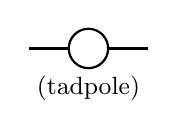
\begin{tikzpicture}[scale=0.5]
\draw[thick] (-1.5,0) -- (-0.5,0);
\draw[thick] (0.5,0) -- (1.5,0);
\draw[thick] (0,0) circle (0.5);
\node at (0,-1) {\small (tadpole)};
\end{tikzpicture}}}
\end{equation}

\textbf{Step 3 (Loop integral):} The one-loop correction to the effective viscosity is:
\begin{equation}
\delta\nu = -A \int_{\Lambda/b}^{\Lambda} \frac{d^d k}{(2\pi)^d} \frac{D_0 k^y}{k^2 \cdot (k^2 + \nu k^2)^2} \approx \frac{A D_0 \Lambda^{y-2}}{\nu^2} \ln b
\end{equation}
where $A$ is a geometric factor from the angular integration.

\textbf{Step 4 (Beta functions):} Taking $b = e^{ds}$ and combining with dimensional scaling:
\begin{align}
\beta_\nu &= (z-2)\nu + \frac{A D_0}{\nu^2 \Lambda^{2-y}} \\
\beta_{D_0} &= (y + 4 - 2z)D_0
\end{align}

\textbf{Fixed point:} Setting $\beta_{D_0} = 0$ determines $z = (y+4)/2$. For Kolmogorov turbulence with constant energy flux, $y = 4$ gives $z = 4$, which is modified by the viscosity correction to yield $z \approx 2$ (the Kolmogorov result $u \sim r^{1/3}$ comes from $h = 1/z$).

\textbf{Physical interpretation:} The fixed point represents the balance between energy injection at large scales and dissipation at small scales. The anomalous corrections come from the nonlinear mode coupling.
\end{workedbox}

\subsection{Functional RG}

The functional RG approach can also be applied to turbulence. This nonperturbative method defines an effective action $\Gamma_k[\mathbf{u}]$ that incorporates fluctuations at scales larger than $1/k$. The Wetterich equation describes its flow:
\begin{equation}
\frac{\partial \Gamma_k}{\partial s} = \frac{1}{2} \mathrm{Tr} \left[ \left( \Gamma_k^{(2)} + R_k \right)^{-1} \frac{\partial R_k}{\partial s} \right]
\end{equation}
where $s = \ln(k_0/k)$ and $R_k$ is the regulator.

\marginnote{The functional RG provides a nonperturbative approach that can handle strong fluctuations.}

%-------------------------------------------------------------------------------
\section{Energy Cascade and Irreversibility}
\label{sec:cascade}
%-------------------------------------------------------------------------------

Turbulence exhibits a characteristic irreversible flow of energy from large to small scales.

\subsection{Energy Flux}

In the inertial range, energy is transferred from scale to scale at a constant rate $\varepsilon$. This cascade is described by the K\'arm\'an-Howarth equation:
\begin{equation}
\frac{\partial}{\partial t}\langle u^2 \rangle = -\frac{2}{r}\frac{\partial}{\partial r}(r^2 \varepsilon_r) + 2\nu \nabla^2 \langle u^2 \rangle
\end{equation}
where $\varepsilon_r$ is the energy flux at scale $r$.

\subsection{Connection to the c-Theorem}

The monotonic decrease of energy to small scales is analogous to the c-theorem in conformal field theory. We can define an ``enstrophy'' (mean-square vorticity in 2D) or other quantities that decrease monotonically along the RG flow.

\marginnote{The energy cascade implements irreversibility in turbulence, just as the c-function decrease implements irreversibility in QFT.}

In 2D turbulence, there is additionally an inverse cascade of energy to large scales, while enstrophy cascades to small scales. This dual cascade structure reflects the additional conserved quantity in 2D.

%-------------------------------------------------------------------------------
\section{Intermittency and Anomalous Dimensions}
\label{sec:intermittency}
%-------------------------------------------------------------------------------

Experimental measurements show systematic deviations from K41 scaling:
\begin{equation}
S_n(r) \sim r^{\zeta_n}, \quad \zeta_n \neq n/3.
\end{equation}

These deviations, called intermittency, indicate that the simple Kolmogorov fixed point does not capture the full physics.

\subsection{Multifractal Models}

The deviation $\Delta_n = \zeta_n - n/3$ represents anomalous dimensions arising from the multi-scale structure of dissipation. Various phenomenological models (log-normal, She-Leveque, etc.) parameterize these corrections.

\marginnote{Intermittency corrections are the turbulent analog of anomalous dimensions in critical phenomena.}

\subsection{RG Interpretation}

From the RG viewpoint, intermittency arises because the Kolmogorov fixed point has relevant or marginally relevant perturbations. The flow does not exactly reach the fixed point, and corrections to scaling appear.

This is analogous to the situation in $\phi^4$ theory where the Wilson-Fisher fixed point has corrections from irrelevant operators that give subleading scaling behavior.

%-------------------------------------------------------------------------------
\section{Analytical Structure of Turbulent Perturbation Theory}
\label{sec:analytical_structure}
%-------------------------------------------------------------------------------

Part II of this book developed the analytical tools for understanding perturbation theory: divergent series, Borel resummation, and resurgence. We now apply these ideas to turbulence, revealing deep connections between perturbative and non-perturbative physics.

\marginnote{The analytical structure of turbulent perturbation theory is largely unexplored---this section outlines what is known and what remains open.}

\subsection{Is Turbulence Perturbation Theory Divergent?}

The perturbation series in both the Yakhot-Orszag and field-theoretic approaches are almost certainly \textbf{factorially divergent} (Gevrey-1), for the same reasons as in QFT (Chapter~\ref{ch:resurgence}).

\textbf{Arguments for factorial divergence:}
\begin{enumerate}
\item \textbf{Combinatorial growth:} At order $n$, the number of Feynman diagrams grows as $n!$ due to the cubic vertex.
\item \textbf{Dyson-like argument:} For negative forcing correlation $D < 0$, the theory is ill-defined (imaginary noise). Hence the series cannot converge in a disk containing both signs.
\item \textbf{Renormalon-like contributions:} Chains of bubble diagrams contribute $\sim n!$ at order $n$.
\end{enumerate}

\textbf{The expected structure:} For the effective viscosity correction:
\begin{equation}
\nu_{\text{eff}} = \nu \left( 1 + \sum_{n=1}^\infty a_n g^n \right), \quad |a_n| \sim C \cdot A^n \cdot n!
\end{equation}
where $g = D_0/(\nu^3 \Lambda^{2-y})$ is the dimensionless coupling.

This factorial growth means the series has \emph{zero radius of convergence}, yet contains physical information extractable via Borel resummation.

\subsection{Borel Transform and Singularities}

Following Chapter~\ref{ch:resurgence}, the Borel transform of the perturbative series is:
\begin{equation}
\hat{\nu}_B(\zeta) = \sum_{n=1}^\infty \frac{a_n}{n!} \zeta^n
\end{equation}

This series \emph{does} converge for $|\zeta| < R$ where $R \sim 1/A$. The singularities of $\hat{\nu}_B(\zeta)$ encode non-perturbative physics.

\marginnote{The Borel singularities in turbulence should correspond to coherent structures or intermittent events.}

\textbf{What are the Borel singularities in turbulence?}

In QFT, Borel singularities arise from:
\begin{itemize}
\item \textbf{Instantons:} Saddle points of the action with finite action
\item \textbf{Renormalons:} Chains of bubble diagrams (IR or UV)
\end{itemize}

For turbulence, we expect analogous structures:
\begin{itemize}
\item \textbf{Coherent structures:} Vortex filaments, sheets, and other organized motions
\item \textbf{Intermittent events:} Rare, intense dissipation events
\item \textbf{IR renormalons:} From the large-scale structure of the cascade
\end{itemize}

\subsection{Instantons in Turbulence}

An \textbf{instanton} in turbulence would be a saddle-point solution of the MSR-JD action~\eqref{eq:msr_action} with finite action.

\textbf{Candidate instantons:}
\begin{enumerate}
\item \textbf{Burgers shocks:} In the Burgers equation, shock solutions are natural saddle points. The ``instanton action'' scales with the shock strength.
\item \textbf{Vortex solutions:} Concentrated vorticity structures (tubes, sheets) that minimize dissipation for given enstrophy.
\item \textbf{Optimal fluctuations:} Solutions that maximize the probability of rare events (large velocity gradients).
\end{enumerate}

\begin{workedbox}[Box 10.D: The Instanton Action for Burgers Turbulence]
\textbf{Setup:} Consider the stochastic Burgers equation $\partial_t u + u \partial_x u = \nu \partial_x^2 u + f$ with Gaussian white noise forcing.

\textbf{The MSR action:}
\begin{equation}
S = \int dx\, dt \left[ \tilde{u}(\partial_t u + u \partial_x u - \nu \partial_x^2 u) - \frac{D}{2} \tilde{u}^2 \right]
\end{equation}

\textbf{Saddle-point equations:}
\begin{align}
\frac{\delta S}{\delta \tilde{u}} &= 0 \quad\Rightarrow\quad \partial_t u + u \partial_x u = \nu \partial_x^2 u + D \tilde{u} \\
\frac{\delta S}{\delta u} &= 0 \quad\Rightarrow\quad -\partial_t \tilde{u} - \partial_x(u \tilde{u}) = \nu \partial_x^2 \tilde{u}
\end{align}

\textbf{Instanton solution:} For a shock-like instanton connecting $u_- \to u_+$:
\begin{equation}
u_{\text{inst}}(x, t) = \frac{u_+ + u_-}{2} - \frac{\Delta u}{2} \tanh\left(\frac{\Delta u \cdot x}{4\nu}\right)
\end{equation}

\textbf{Instanton action:}
\begin{equation}
S_{\text{inst}} \sim \frac{(\Delta u)^3}{D \nu}
\end{equation}

\textbf{Physical interpretation:} The instanton describes the optimal (most probable) way to create a shock with velocity jump $\Delta u$. The probability of such events is $\sim e^{-S_{\text{inst}}}$, giving the tail of the velocity gradient PDF.
\end{workedbox}

\subsection{Resurgence and Intermittency}

\marginnote{A speculative but tantalizing possibility: intermittency corrections are encoded in the resurgent structure of the perturbation series.}

The most intriguing possibility is that \textbf{intermittency corrections} arise from resurgent structure---the same mechanism that connects perturbative and non-perturbative physics in QFT.

\textbf{The hypothesis:}
\begin{itemize}
\item The perturbative series for scaling exponents $\zeta_n$ diverges factorially
\item The Borel singularities encode intermittent events (coherent structures)
\item The anomalous dimensions $\Delta_n = \zeta_n - n/3$ arise from resurgent contributions
\item Stokes phenomena across different regimes (inertial range boundaries) modify the exponents
\end{itemize}

\textbf{Evidence (circumstantial):}
\begin{enumerate}
\item Intermittency is associated with rare, intense events---precisely what instantons describe
\item The She-Leveque model involves a geometric series $(2/3)^{n/3}$ suggestive of instanton-anti-instanton contributions
\item The multifractal structure implies multiple saddle points contributing to different moments
\end{enumerate}

\textbf{Open problems:}
\begin{enumerate}
\item Compute the Borel singularities of the turbulence perturbation series explicitly
\item Identify the instanton configurations in 3D Navier-Stokes
\item Derive the She-Leveque (or other intermittency) exponents from resurgence
\item Understand the role of Stokes phenomena at the boundaries of the inertial range
\end{enumerate}

This remains an open frontier---a synthesis of Part II's analytical methods with turbulence theory that could yield new insights into intermittency.

\subsection{Transseries for Turbulence}

If the perturbation series is resurgent, the complete answer should be a \textbf{transseries}:
\begin{equation}
\nu_{\text{eff}}(g) = \sum_{n=0}^\infty a_n g^n + \sum_{k=1}^\infty \sigma^k e^{-k S_0/g} \sum_{n=0}^\infty b_{k,n} g^n + \cdots
\end{equation}
where $S_0$ is the instanton action and $\sigma$ is a transseries parameter.

\marginnote{Transseries provide the complete non-perturbative answer, incorporating both perturbative and instanton contributions.}

The non-perturbative sectors ($e^{-S/g}$ terms) correspond to:
\begin{itemize}
\item $k = 1$: Single instanton (isolated coherent structure)
\item $k = 2$: Instanton-anti-instanton pairs
\item Higher $k$: Multi-instanton configurations
\end{itemize}

The transseries structure would encode the full statistics of turbulence, including the tails of probability distributions that determine intermittency.

%-------------------------------------------------------------------------------
\section{Application: Shock Waves in Burgers}
\label{sec:shock}
%-------------------------------------------------------------------------------

As a concrete application, consider shock formation in the inviscid Burgers equation.

\subsection{Method of Characteristics}

The inviscid Burgers equation $u_t + uu_x = 0$ can be solved by characteristics. For smooth initial data $u(x, 0) = u_0(x)$, the solution develops shocks in finite time when characteristics cross.

\subsection{Intermediate Asymptotics}

After shock formation, the solution enters an intermediate asymptotic regime where the specific initial conditions are forgotten but the overall structure of shocks persists.

The similarity solution for a single shock is
\begin{equation}
u(x, t) = \frac{x}{t}
\end{equation}
for $|x| < s(t)$ where $s(t)$ is the shock position. This is a self-similar solution of the first kind.

\subsection{Viscous Corrections}

With small viscosity $\nu > 0$, the shock has finite width $\sim \nu/\Delta u$ where $\Delta u$ is the velocity jump. The shock structure is
\begin{equation}
u(x, t) = \frac{u_L + u_R}{2} - \frac{\Delta u}{2}\tanh\left(\frac{\Delta u (x - st)}{4\nu}\right)
\end{equation}
where $u_L, u_R$ are the velocities on either side and $s = (u_L + u_R)/2$ is the shock speed.

\marginnote{The shock width $\sim \nu$ is the dissipation scale, analogous to the Kolmogorov scale $\eta$ in turbulence.}

This solution illustrates how small-scale physics (viscosity) regularizes the large-scale dynamics (shock), precisely the multi-scale structure that the RG is designed to handle.

%-------------------------------------------------------------------------------
\section{Non-Relativistic Conformal Symmetry}
\label{sec:fluid_conformal}
%-------------------------------------------------------------------------------

The equations of fluid mechanics possess a remarkable symmetry structure that goes far beyond simple scale invariance. Under appropriate conditions, they exhibit \textbf{non-relativistic conformal symmetry}, governed by the \textbf{Schrödinger group} and its generalizations. This symmetry provides powerful constraints analogous to those in relativistic CFT~\cite{Henkel2006, Hassaine2009, Horvathy2010}.

\subsection{The Schrödinger Group}

\marginnote{The Schrödinger group extends Galilean symmetry to include dilations and special conformal transformations.}

The Schrödinger group is the maximal kinematical group of the free Schrödinger equation $i\partial_t\psi = -\frac{1}{2m}\nabla^2\psi$. It includes:
\begin{enumerate}
\item \textbf{Spatial translations:} $H_i: x_i \to x_i + a_i$
\item \textbf{Time translation:} $P: t \to t + b$
\item \textbf{Rotations:} $M_{ij}: x_i \to R_{ij}x_j$
\item \textbf{Galilean boosts:} $G_i: x_i \to x_i + v_i t$, $\psi \to e^{imv\cdot x - \frac{1}{2}mv^2t}\psi$
\item \textbf{Dilation:} $D: x \to \lambda x$, $t \to \lambda^z t$
\item \textbf{Special conformal:} $K: t \to t/(1-ct)$, $x \to x/(1-ct)$
\end{enumerate}

The \textbf{dynamical exponent} $z$ characterizes how time scales relative to space. For the free Schrödinger equation, $z = 2$.

\textbf{Lie algebra structure.} The generators satisfy:
\begin{align}
[D, H_i] &= H_i, \quad [D, P] = zP, \quad [D, G_i] = (1-z)G_i \\
[D, K] &= -zK, \quad [K, P] = D, \quad [K, H_i] = G_i
\end{align}

\subsection{Conformal Galilei Algebra}

A generalization is the \textbf{Conformal Galilei Algebra} (CGA), which exists for any rational $z = 2/N$ with $N \in \mathbb{Z}^+$~\cite{Horvathy2010}. The standard Schrödinger algebra corresponds to $N = 1$ (so $z = 2$).

\begin{workedbox}[Box 10.3: Non-Relativistic Conformal Ward Identities]
\textbf{Correlation functions in Schrödinger-invariant theories:}

Just as relativistic conformal symmetry constrains correlation functions, the Schrödinger group constrains \textbf{non-relativistic correlation functions}. For primary fields $\phi_\alpha$ with scaling dimension $\Delta_\alpha$ and ``mass'' (or particle number) $m_\alpha$:

\textbf{Two-point function:}
\begin{equation}
\langle\phi_1(x_1, t_1)\phi_2(x_2, t_2)\rangle = \delta_{\Delta_1,\Delta_2}\delta_{m_1+m_2,0} \cdot \frac{f\left(\frac{|x_{12}|^2}{t_{12}}\right)}{t_{12}^{\Delta_1/z}}
\end{equation}
where $x_{12} = x_1 - x_2$ and $t_{12} = t_1 - t_2$. The function $f$ is constrained by special conformal invariance.

\textbf{Three-point function:}
\begin{equation}
\langle\phi_1\phi_2\phi_3\rangle = \delta_{m_1+m_2+m_3,0} \cdot t_{12}^{-a}t_{23}^{-b}t_{13}^{-c} \cdot F(\xi_1, \xi_2, \xi_3)
\end{equation}
where $a, b, c$ are determined by dimensions and $\xi_i$ are conformally invariant combinations of coordinates.

\textbf{RG significance:} These constraints determine correlation functions at non-relativistic fixed points, exactly as CFT constraints determine relativistic fixed-point correlators.
\end{workedbox}

\subsection{Application to Fluid Mechanics}

The Navier-Stokes equations enjoy scale invariance for appropriate forcing. More remarkably, the inviscid Euler equations and certain diffusion equations possess the \textbf{full Schrödinger symmetry}~\cite{Hassaine2009}.

\textbf{The incompressible Euler equations:}
\begin{equation}
\partial_t u_i + u_j\partial_j u_i = -\partial_i p, \quad \partial_i u_i = 0
\end{equation}
These are invariant under the Schrödinger group with $z = 1$ (meaning $t \to \lambda t$ and $x \to \lambda x$ scale equally), provided we transform:
\begin{equation}
u_i \to \lambda^{-z+1} u_i, \quad p \to \lambda^{-2z+2} p
\end{equation}

\textbf{Diffusion and PME connection:} The linear diffusion equation $\partial_t \rho = D\nabla^2\rho$ has Schrödinger symmetry with $z = 2$. The Porous Medium Equation (Chapter~\ref{ch:fixed_points}) breaks this to scale invariance alone, with anomalous exponents arising from the nonlinearity.

\begin{workedbox}[Box 10.4: Group-Theoretic Construction of Self-Similar Solutions]
\textbf{Symmetry-guided solution ansatz:}

Given a PDE with Schrödinger symmetry, group theory provides a systematic construction of self-similar solutions:

\begin{enumerate}
\item \textbf{Identify the symmetry algebra} $\mathfrak{g}$ (e.g., Schrödinger algebra)
\item \textbf{Find invariant combinations} under the one-parameter subgroup generated by $D + \alpha K$ for various $\alpha$
\item \textbf{Reduce the PDE} by assuming the solution depends only on these invariants
\item \textbf{Solve the reduced ODE} to obtain the scaling function
\end{enumerate}

\textbf{Example: Barenblatt solution from symmetry.}

For the PME $\partial_t \rho = \nabla \cdot (\rho^m \nabla\rho)$, the scaling symmetry demands:
\begin{equation}
\rho(x, t) = t^{-\alpha}f(\xi), \quad \xi = x/t^\beta
\end{equation}
where $\alpha$ and $\beta$ are fixed by requiring the ansatz to solve the equation.

This is precisely the dimensional analysis approach from Chapter~\ref{ch:fixed_points}, now understood as representation theory of the symmetry group.
\end{workedbox}

\subsection{Aging and Time-Translation Breaking}

A significant extension concerns systems that break time-translation symmetry---relevant for glassy dynamics and non-equilibrium systems~\cite{Henkel2006}. These systems exhibit \textbf{aging}: their properties depend on the ``age'' (time since preparation), not just on time differences.

The symmetry algebra becomes the \textbf{aging algebra}, where the time-translation generator $P$ is absent. Correlation functions depend on both times $t_1$ and $t_2$ separately, not just $t_1 - t_2$:
\begin{equation}
C(t_1, t_2) = t_1^{-\lambda/z}f_C(t_1/t_2)
\end{equation}
where $\lambda$ is the autoresponse exponent. This structure has been confirmed in numerical simulations of aging systems.

%-------------------------------------------------------------------------------
\section{Connection to the Geometric Framework}
\label{sec:fluids_geometry}
%-------------------------------------------------------------------------------

We now make explicit the connection to Part I.

\subsection{Theory Space for Fluids}

The couplings that parametrize theory space for fluid dynamics include the viscosity $\nu$ (or equivalently the Reynolds number $Re$), parameters characterizing the forcing spectrum such as its amplitude and spatial structure, and any additional dimensionless parameters that enter the problem. For homogeneous isotropic turbulence with power-law forcing, the essential parameters reduce to the effective viscosity and the forcing exponent.

The RG flow describes how the effective viscosity changes as we coarse-grain:
\begin{equation}
\frac{\dd \nu_{\text{eff}}}{\dd s} = \beta_\nu(\nu_{\text{eff}}, \ldots).
\end{equation}
At the Kolmogorov fixed point, $\beta_\nu = 0$ and the effective viscosity has reached a scale-invariant value. The fixed-point theory describes the universal scaling behavior in the inertial range.

\subsection{Self-Similarity from Equivariance}

The self-similar solutions of Section~\ref{sec:burgers} arise from the scale covariance requirement discussed in Chapter~\ref{ch:rg_geometry}. If the solution is to be independent of the arbitrary choice of length scale, it must take the self-similar form.

The scaling exponents emerge as eigenvalues of the RG transformation, exactly as in Chapter~\ref{ch:fixed_points}.

\subsection{Connection to the Three Canonical Examples}

Turbulence connects to each of the three canonical examples from Part I:

\marginnote{Turbulence is a particularly rich application, drawing on all three canonical examples.}

\textbf{Anharmonic oscillator parallel.} The velocity field expansion encounters secular growth from mode coupling. The effective viscosity ``runs'' with scale, curing the divergences much as the running frequency cures secular terms in the oscillator.

\textbf{$\phi^4$ theory parallel.} Kolmogorov scaling is a non-trivial fixed point analogous to Wilson-Fisher. The deviations from dimensional analysis (the Kolmogorov $-5/3$ exponent vs.\ the dimensional prediction) parallel the Wilson-Fisher exponents differing from mean-field values.

\textbf{PME parallel.} Intermittency corrections are anomalous dimensions in the same sense as the PME: the structure function exponents $\zeta_n$ cannot be predicted from dimensional analysis alone but must be computed from the nonlinear dynamics. This is second-kind self-similarity applied to turbulence.

%-------------------------------------------------------------------------------
\section{Synthesis: A Unified View of Turbulence RG}
\label{sec:synthesis}
%-------------------------------------------------------------------------------

We conclude by synthesizing the various approaches within the unified framework of algebra, geometry, and analysis.

\subsection{Comparison of Approaches}

The following table summarizes how each approach realizes the geometric RG framework:

\begin{center}
\renewcommand{\arraystretch}{1.4}
\small
\begin{tabular}{p{2.2cm}p{2.5cm}p{2.8cm}p{2.5cm}p{2.5cm}}
\toprule
\textbf{Approach} & \textbf{Theory Space} & \textbf{Beta Function} & \textbf{Fixed Point} & \textbf{Expansion} \\
\midrule
Yakhot-Orszag & $(\nu, D_0, y)$ & Direct mode elimination & Kolmogorov & $\varepsilon = y - y_c$ \\
\addlinespace
McComb & $\nu_{\text{eff}}(k)$ & Iterative averaging & Scale-indep.\ $\nu$ & Numerical \\
\addlinespace
MSR-JD Field Theory & All operators & Feynman diagrams & IR fixed point & Loop expansion \\
\addlinespace
Kraichnan DIA & (Reinterpreted) & Flow from Gaussian & Gaussian FP & Self-consistent \\
\addlinespace
Functional RG & $\Gamma_k[u]$ & Wetterich equation & Non-perturbative & Truncation \\
\bottomrule
\end{tabular}
\end{center}

\marginnote{Each approach makes different choices about what constitutes theory space and how to implement coarse-graining.}

\subsection{The Algebraic Perspective}

\textbf{Lie group structure:} All approaches share the same underlying Lie group---the dilation group acting on length scales. The differences lie in:
\begin{itemize}
\item How the group acts on the chosen theory space
\item The representation of the Lie algebra generator (beta function)
\item Which truncation or approximation is used
\end{itemize}

\textbf{Lie algebra:} The beta function $\boldsymbol{\beta} = \beta^i \partial/\partial g^i$ generates the RG flow in each case:
\begin{itemize}
\item Yakhot-Orszag: Finite-dimensional Lie algebra on $(\nu, D_0)$
\item Field-theoretic: Infinite-dimensional on the space of operators
\item Functional RG: Functional derivative on the effective action space
\end{itemize}

\subsection{The Geometric Perspective}

\textbf{Fixed point structure:}
\begin{center}
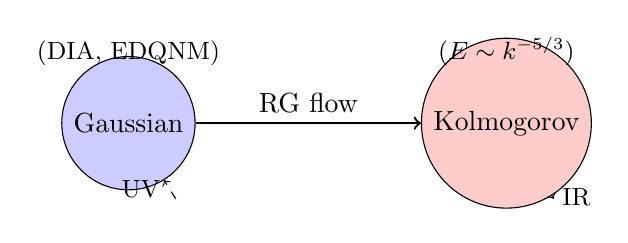
\begin{tikzpicture}[scale=1.2]
\node[circle, draw, fill=blue!20] (G) at (0, 0) {Gaussian};
\node[circle, draw, fill=red!20] (K) at (4, 0) {Kolmogorov};
\node[above] at (0, 0.5) {\small (DIA, EDQNM)};
\node[above] at (4, 0.5) {\small ($E \sim k^{-5/3}$)};
\draw[->, thick] (G) -- (K) node[midway, above] {RG flow};
\draw[->, dashed] (0.5, -0.8) -- (G) node[midway, left] {\small UV};
\draw[->, dashed] (K) -- (4.5, -0.8) node[midway, right] {\small IR};
\end{tikzpicture}
\end{center}

The geometric picture unifies the approaches:
\begin{itemize}
\item \textbf{UV (small scales):} Gaussian-like behavior, DIA-type closures work
\item \textbf{IR (large scales):} Flow toward Kolmogorov fixed point
\item \textbf{Intermittency:} Corrections from operators near marginality
\end{itemize}

\textbf{Stability and universality:} The Kolmogorov fixed point is an \emph{attractor} with a basin of attraction defining the universality class of fully developed turbulence. Different forcing mechanisms, boundary conditions, and initial conditions flow to the same fixed point, explaining the universality of the $-5/3$ spectrum.

\subsection{The Analytical Perspective}

\textbf{Perturbation theory:}
\begin{itemize}
\item All approaches involve perturbation expansions (explicit or implicit)
\item The series are generically factorially divergent (Gevrey-1)
\item Borel resummation is needed for quantitative predictions
\end{itemize}

\textbf{Non-perturbative physics:}
\begin{itemize}
\item Instantons (coherent structures) contribute $\sim e^{-S/g}$
\item Intermittency may arise from resurgent structure
\item Transseries provide the complete answer
\end{itemize}

\textbf{Open frontier:} The analytical structure of turbulence perturbation theory remains largely unexplored. Applying Part II's resurgence methods could yield new insights into intermittency.

\subsection{Key Takeaways}

\begin{enumerate}
\item \textbf{Multiple approaches, one framework:} Yakhot-Orszag, field-theoretic, and functional RG are different implementations of the same geometric RG structure.

\item \textbf{Closures fit the picture:} Kraichnan's DIA and other closures correspond to the Gaussian fixed point, with corrections describing flow toward Kolmogorov.

\item \textbf{Kolmogorov is universal:} The $-5/3$ spectrum is the signature of an IR attractive fixed point, explaining why diverse turbulent flows share this scaling.

\item \textbf{Intermittency is anomalous:} Deviations from K41 are anomalous dimensions, potentially connected to resurgent/non-perturbative physics.

\item \textbf{Much remains open:} The analytical structure (Borel singularities, instantons, transseries) of turbulence is a frontier for future research.
\end{enumerate}

%-------------------------------------------------------------------------------
\section*{Exercises}
\addcontentsline{toc}{section}{Exercises}
%-------------------------------------------------------------------------------

\begin{enumerate}
\item \textbf{Kolmogorov scales.} For turbulent flow with kinematic viscosity $\nu$ and energy dissipation rate $\varepsilon$:
\begin{enumerate}
\item Derive the Kolmogorov length scale $\eta = (\nu^3/\varepsilon)^{1/4}$ from dimensional analysis.
\item Derive the Kolmogorov velocity scale $u_\eta = (\nu\varepsilon)^{1/4}$.
\item Show that the Reynolds number based on Kolmogorov scales is $Re_\eta = u_\eta\eta/\nu = 1$.
\end{enumerate}

\item \textbf{K41 scaling.} Kolmogorov's 1941 theory predicts $S_n(r) \sim (\varepsilon r)^{n/3}$.
\begin{enumerate}
\item Derive this scaling from dimensional analysis, assuming $S_n$ depends only on $\varepsilon$ and $r$.
\item Show that the energy spectrum $E(k) \sim \varepsilon^{2/3}k^{-5/3}$ follows from $S_2(r) \sim (\varepsilon r)^{2/3}$.
\item Discuss what physical assumptions underlie K41 theory.
\end{enumerate}

\item \textbf{Burgers equation.} For the inviscid Burgers equation $u_t + uu_x = 0$:
\begin{enumerate}
\item Show that the method of characteristics gives $u = u_0(x - ut)$ implicitly.
\item Derive the shock formation time for initial condition $u_0(x) = -\sin x$.
\item Find the self-similar solution $u(x,t) = f(x/t)/t$ and determine $f$.
\end{enumerate}

\item \textbf{Energy cascade.} In 3D turbulence:
\begin{enumerate}
\item Explain why energy cascades from large to small scales (direct cascade).
\item In 2D turbulence, explain why energy undergoes an inverse cascade.
\item How does enstrophy (mean-square vorticity) behave in 2D?
\end{enumerate}

\item \textbf{(Challenge) Intermittency.} The She-Leveque model predicts $\zeta_n = n/9 + 2(1 - (2/3)^{n/3})$.
\begin{enumerate}
\item Verify that $\zeta_3 = 1$ (exact result from the K\'arm\'an-Howarth equation).
\item Compare $\zeta_2$ and $\zeta_6$ with K41 predictions.
\item Discuss the physical origin of intermittency corrections.
\end{enumerate}
\end{enumerate}

%-------------------------------------------------------------------------------
\subsection*{Solutions}
%-------------------------------------------------------------------------------

\begin{solutionbox}{Exercise 10.1: Kolmogorov Scales}
\textbf{(a) Length scale.}

We seek the scale where viscous forces balance inertial forces. The only parameters are:
\begin{itemize}
\item $\nu$ (kinematic viscosity): $[\nu] = L^2/T$
\item $\varepsilon$ (energy dissipation rate): $[\varepsilon] = L^2/T^3$
\end{itemize}

For a length scale $\eta = \nu^a \varepsilon^b$:
\begin{equation}
L = L^{2a} T^{-a} \cdot L^{2b} T^{-3b} = L^{2a+2b} T^{-a-3b}
\end{equation}

This gives: $2a + 2b = 1$ and $a + 3b = 0$. Solving: $a = 3/4$, $b = -1/4$.
\begin{equation}
\boxed{\eta = \left(\frac{\nu^3}{\varepsilon}\right)^{1/4}}
\end{equation}

\textbf{(b) Velocity scale.}

For $u_\eta = \nu^c \varepsilon^d$:
\begin{equation}
L/T = L^{2c+2d} T^{-c-3d}
\end{equation}

This gives: $2c + 2d = 1$ and $c + 3d = 1$. Solving: $c = 1/4$, $d = 1/4$.
\begin{equation}
\boxed{u_\eta = (\nu\varepsilon)^{1/4}}
\end{equation}

\textbf{(c) Reynolds number.}
\begin{equation}
Re_\eta = \frac{u_\eta \eta}{\nu} = \frac{(\nu\varepsilon)^{1/4} \cdot (\nu^3/\varepsilon)^{1/4}}{\nu} = \frac{(\nu^4)^{1/4}}{\nu} = \frac{\nu}{\nu} = 1
\end{equation}

This confirms that the Kolmogorov scale is where viscous and inertial effects are balanced.
\end{solutionbox}

\begin{solutionbox}{Exercise 10.2: K41 Scaling}
\textbf{(a) Structure function scaling.}

Assume $S_n(r) = \langle|\delta u|^n\rangle$ depends only on $\varepsilon$ and $r$ in the inertial range.

Dimensions: $[S_n] = (L/T)^n$, $[\varepsilon] = L^2/T^3$, $[r] = L$.

Let $S_n = \varepsilon^a r^b$:
\begin{equation}
L^n T^{-n} = L^{2a} T^{-3a} \cdot L^b = L^{2a+b} T^{-3a}
\end{equation}

Matching: $3a = n$ and $2a + b = n$. So $a = n/3$ and $b = n/3$.
\begin{equation}
\boxed{S_n(r) \sim (\varepsilon r)^{n/3}}
\end{equation}

\textbf{(b) Energy spectrum.}

The second-order structure function relates to the energy spectrum via:
\begin{equation}
S_2(r) \sim \int_0^\infty E(k)(1 - \cos kr)\,dk \sim \int_0^{1/r} E(k)\,dk
\end{equation}

If $S_2(r) \sim \varepsilon^{2/3} r^{2/3}$, then differentiating:
\begin{equation}
\frac{dS_2}{dr} \sim E(1/r) \cdot \frac{1}{r^2} \sim \varepsilon^{2/3} r^{-1/3}
\end{equation}

So $E(k) \sim \varepsilon^{2/3} k^{-5/3}$.

\textbf{(c) Physical assumptions.}

K41 assumes:
\begin{itemize}
\item \textit{Locality}: Statistics at scale $r$ depend only on $\varepsilon$ (constant energy flux)
\item \textit{Isotropy}: Homogeneous, isotropic turbulence
\item \textit{Scale separation}: $\eta \ll r \ll L$ (inertial range)
\item \textit{Statistical stationarity}: Time-averaged quantities are constant
\end{itemize}
\end{solutionbox}

\begin{solutionbox}{Exercise 10.3: Burgers Equation}
\textbf{(a) Method of characteristics.}

Along characteristics $dx/dt = u$, we have $du/dt = 0$. So $u = \text{const}$ along each characteristic, and characteristics are straight lines:
\begin{equation}
x = x_0 + u_0(x_0) \cdot t
\end{equation}

Inverting: the value $u$ at $(x,t)$ equals $u_0(x_0)$ where $x_0$ satisfies $x = x_0 + u_0(x_0)t$, i.e., $u = u_0(x - ut)$.

\textbf{(b) Shock formation time.}

For $u_0(x) = -\sin x$, characteristics are $x = x_0 - t\sin x_0$.

Characteristics cross when $\partial x/\partial x_0 = 0$:
\begin{equation}
\frac{\partial x}{\partial x_0} = 1 - t\cos x_0 = 0 \quad\Rightarrow\quad t = \frac{1}{\cos x_0}
\end{equation}

The first crossing occurs at $x_0 = 0$ where $\cos x_0 = 1$, giving:
\begin{equation}
\boxed{t_{\text{shock}} = 1}
\end{equation}

\textbf{(c) Self-similar solution.}

Substitute $u(x,t) = f(\xi)/t$ where $\xi = x/t$ into $u_t + uu_x = 0$:
\begin{equation}
-\frac{f}{t^2} - \frac{\xi f'}{t^2} + \frac{f}{t}\cdot\frac{f'}{t^2} = 0
\end{equation}

Multiplying by $t^2$: $-f - \xi f' + ff'/t = 0$. For large $t$, the last term dominates balance requires $ff' \approx 0$, but for the N-wave solution:
\begin{equation}
f(\xi) = \xi \quad\text{for } |\xi| < \xi_s
\end{equation}
giving $u = x/t$ (the ``sawtooth'' or N-wave solution).
\end{solutionbox}

\begin{solutionbox}{Exercise 10.4: Energy Cascade}
\textbf{(a) Direct cascade in 3D.}

In 3D, vortex stretching transfers energy to smaller scales:
\begin{itemize}
\item Large eddies break into smaller ones through nonlinear interactions
\item Vorticity is amplified by stretching: $D\omega/Dt = (\omega\cdot\nabla)\mathbf{u}$
\item Energy is conserved in the inertial range and dissipated only at the smallest scales
\end{itemize}

The cascade direction is from large to small scales because energy is injected at large scales and removed at small scales by viscosity.

\textbf{(b) Inverse cascade in 2D.}

In 2D, there is no vortex stretching (vorticity is a scalar). Two conserved quantities exist:
\begin{itemize}
\item Energy: $E = \frac{1}{2}\langle u^2 \rangle$
\item Enstrophy: $\Omega = \frac{1}{2}\langle \omega^2 \rangle$
\end{itemize}

If energy were to cascade to small scales, enstrophy would have to cascade even faster (since $\Omega \sim k^2 E$). But enstrophy dissipation is limited, forcing energy to cascade to large scales instead.

\textbf{(c) Enstrophy in 2D.}

Enstrophy undergoes a \textit{direct cascade} to small scales, with spectrum $\Omega(k) \sim \eta^{2/3} k^{-1}$ where $\eta$ is the enstrophy dissipation rate.

The dual cascade structure:
\begin{itemize}
\item Energy: inverse cascade, $E(k) \sim \varepsilon^{2/3} k^{-5/3}$ for $k < k_f$
\item Enstrophy: direct cascade, $\Omega(k) \sim \eta^{2/3} k^{-3}$ for $k > k_f$
\end{itemize}
where $k_f$ is the forcing wavenumber.
\end{solutionbox}

\begin{solutionbox}{Exercise 10.5: Intermittency (Challenge)}
\textbf{(a) Verify $\zeta_3 = 1$.}

From the She-Leveque formula:
\begin{equation}
\zeta_3 = \frac{3}{9} + 2\left(1 - \left(\frac{2}{3}\right)^1\right) = \frac{1}{3} + 2 \times \frac{1}{3} = \frac{1}{3} + \frac{2}{3} = 1 \quad\checkmark
\end{equation}

This is exact due to the K\'arm\'an-Howarth relation, which gives $S_3(r) = -\frac{4}{5}\varepsilon r$ in the inertial range.

\textbf{(b) Comparison with K41.}

K41 predicts $\zeta_n^{K41} = n/3$. She-Leveque (SL) predicts $\zeta_n^{SL} = n/9 + 2(1 - (2/3)^{n/3})$.

For $n = 2$:
\begin{equation}
\zeta_2^{K41} = 2/3 \approx 0.667, \qquad \zeta_2^{SL} = \frac{2}{9} + 2(1 - (2/3)^{2/3}) \approx 0.696
\end{equation}

For $n = 6$:
\begin{equation}
\zeta_6^{K41} = 2, \qquad \zeta_6^{SL} = \frac{6}{9} + 2(1 - (2/3)^2) = \frac{2}{3} + 2 \times \frac{5}{9} = 1.78
\end{equation}

Experiments confirm $\zeta_6 \approx 1.78$, validating intermittency corrections.

\textbf{(c) Physical origin.}

Intermittency arises from the \textit{multifractal structure} of dissipation:
\begin{itemize}
\item Dissipation is not uniform but concentrated in filaments and sheets
\item Different moments probe different regions of this distribution
\item The local dissipation rate $\varepsilon_r$ at scale $r$ fluctuates strongly
\end{itemize}

The She-Leveque model assumes dissipation is concentrated in quasi-1D filaments, giving the $(2/3)^{n/3}$ factor from the dimension deficit.
\end{solutionbox}

%-------------------------------------------------------------------------------
\section*{Summary}
\addcontentsline{toc}{section}{Summary}
%-------------------------------------------------------------------------------

\begin{summarybox}{Chapter 10: Turbulence and Fluid Dynamics}

\summaryheader{The Geometric Framework (Algebra)}
\begin{itemize}
\item \textbf{Theory space:} $\MM = \{(\nu_{\text{eff}}, D_0, y, \ldots)\}$ or full operator space
\item \textbf{Beta functions:} $\beta_\nu = (z-2)\nu + AD_0/\nu^2$, $\beta_D = (y+4-2z)D_0$
\item \textbf{Fixed points:} Kolmogorov (interacting), DIA (Gaussian)
\item \textbf{Stability matrix:} Eigenvalues give scaling dimensions
\item \textbf{Dimensionless coupling:} $g = D_0/(\nu^3 \Lambda^{2-y})$
\end{itemize}

\summaryheader{Taxonomy of Approaches}
\begin{itemize}
\item \textbf{Direct methods:} Yakhot-Orszag, McComb (no path integral)
\item \textbf{Field-theoretic:} MSR-JD formalism (path integral with response fields)
\item \textbf{Closures as fixed points:} DIA $\approx$ Gaussian FP, flow toward Kolmogorov
\item \textbf{Unifying insight:} All methods implement same Lie group structure differently
\end{itemize}

\summaryheader{Analytical Structure (Part II Connection)}
\begin{itemize}
\item \textbf{Divergent series:} Perturbation theory is Gevrey-1 (factorially divergent)
\item \textbf{Borel singularities:} Correspond to coherent structures, intermittent events
\item \textbf{Instantons:} Shocks (Burgers), vortex filaments (Navier-Stokes)
\item \textbf{Open frontier:} Resurgence may explain intermittency corrections
\end{itemize}

\summaryheader{Key Physical Insights}
\begin{itemize}
\item \textbf{Kolmogorov scaling} = IR attractive fixed point ($E(k) \sim k^{-5/3}$)
\item \textbf{DIA failure} ($k^{-3/2}$) = Gaussian FP, not true turbulence
\item \textbf{Intermittency} = anomalous dimensions, possibly resurgent origin
\item \textbf{Energy cascade} = irreversible RG flow (c-theorem analog)
\end{itemize}

\end{summarybox}

